\chapter{Diversité} \label{ch:DIV}

\section{Mesures et méthodologie}

L'objectif du travail est de quantifier l'impacte de la diversité sur la propagation de pandémies. Cette section est dédié à la prises de mesures avec des niveaux de diversité différents et d'en constater les résultats. Afin de ne pas trop complexifier le modèle au delà des simulations SIR, nous ne modifions que le paramètre de diversité, nombre de mouvements ainsi que la charge virale. D'autres paramètres du modèle pourraient être étudié mais ce chapitre ne les explore pas.\\

La recherche sur la diversité est découpée en trois parties. La première explore l'impacte de la diversité sur des simulations à propagation de pandémie rapide. Dans ce cas nous observons donc la réaction de la diversité sur l'immunisation des individus déjà contaminés. La seconde cherche à déterminer le taux de simulations qui développent une pandémie, c'est-à-dire le nombre de simulations qui réussissent ou échouent à développer une pandémie en fonction de la diversité de la population. La troisième tente d'observer des pandémies partielles qui ne parviennent pas à contaminer toute la population.\\


\section{Pandémies totales}

Le premier chapitre est une observation de l'impacte de la diversité sur des systèmes de densité $1/16$ au mélange parfait. L'analyse est purement qualitative et permet de visualiser le comportement du mécanisme d'immunisation en fonction du facteur de diversité.\\

L'unique simulation étudié est de taille $1264 \times 1264$ avec une population de $10^5$. La charge virale est définie à $1$ et la diversité est de $4,8,16,32$. Les génomes de tous les individus sont initialement identiques. Dans cette configuration, les agents pathogènes ont la meilleure compatibilité possible et sont donc les plus virulents. La figure suivante montre des simulations qui intègrent de la diverstié sur les génomes des individus afin de réduire la virulence des pathogènes.

\newpage

\begin{figure}[h]
	\centering
	\captionsetup{justification=centering}
	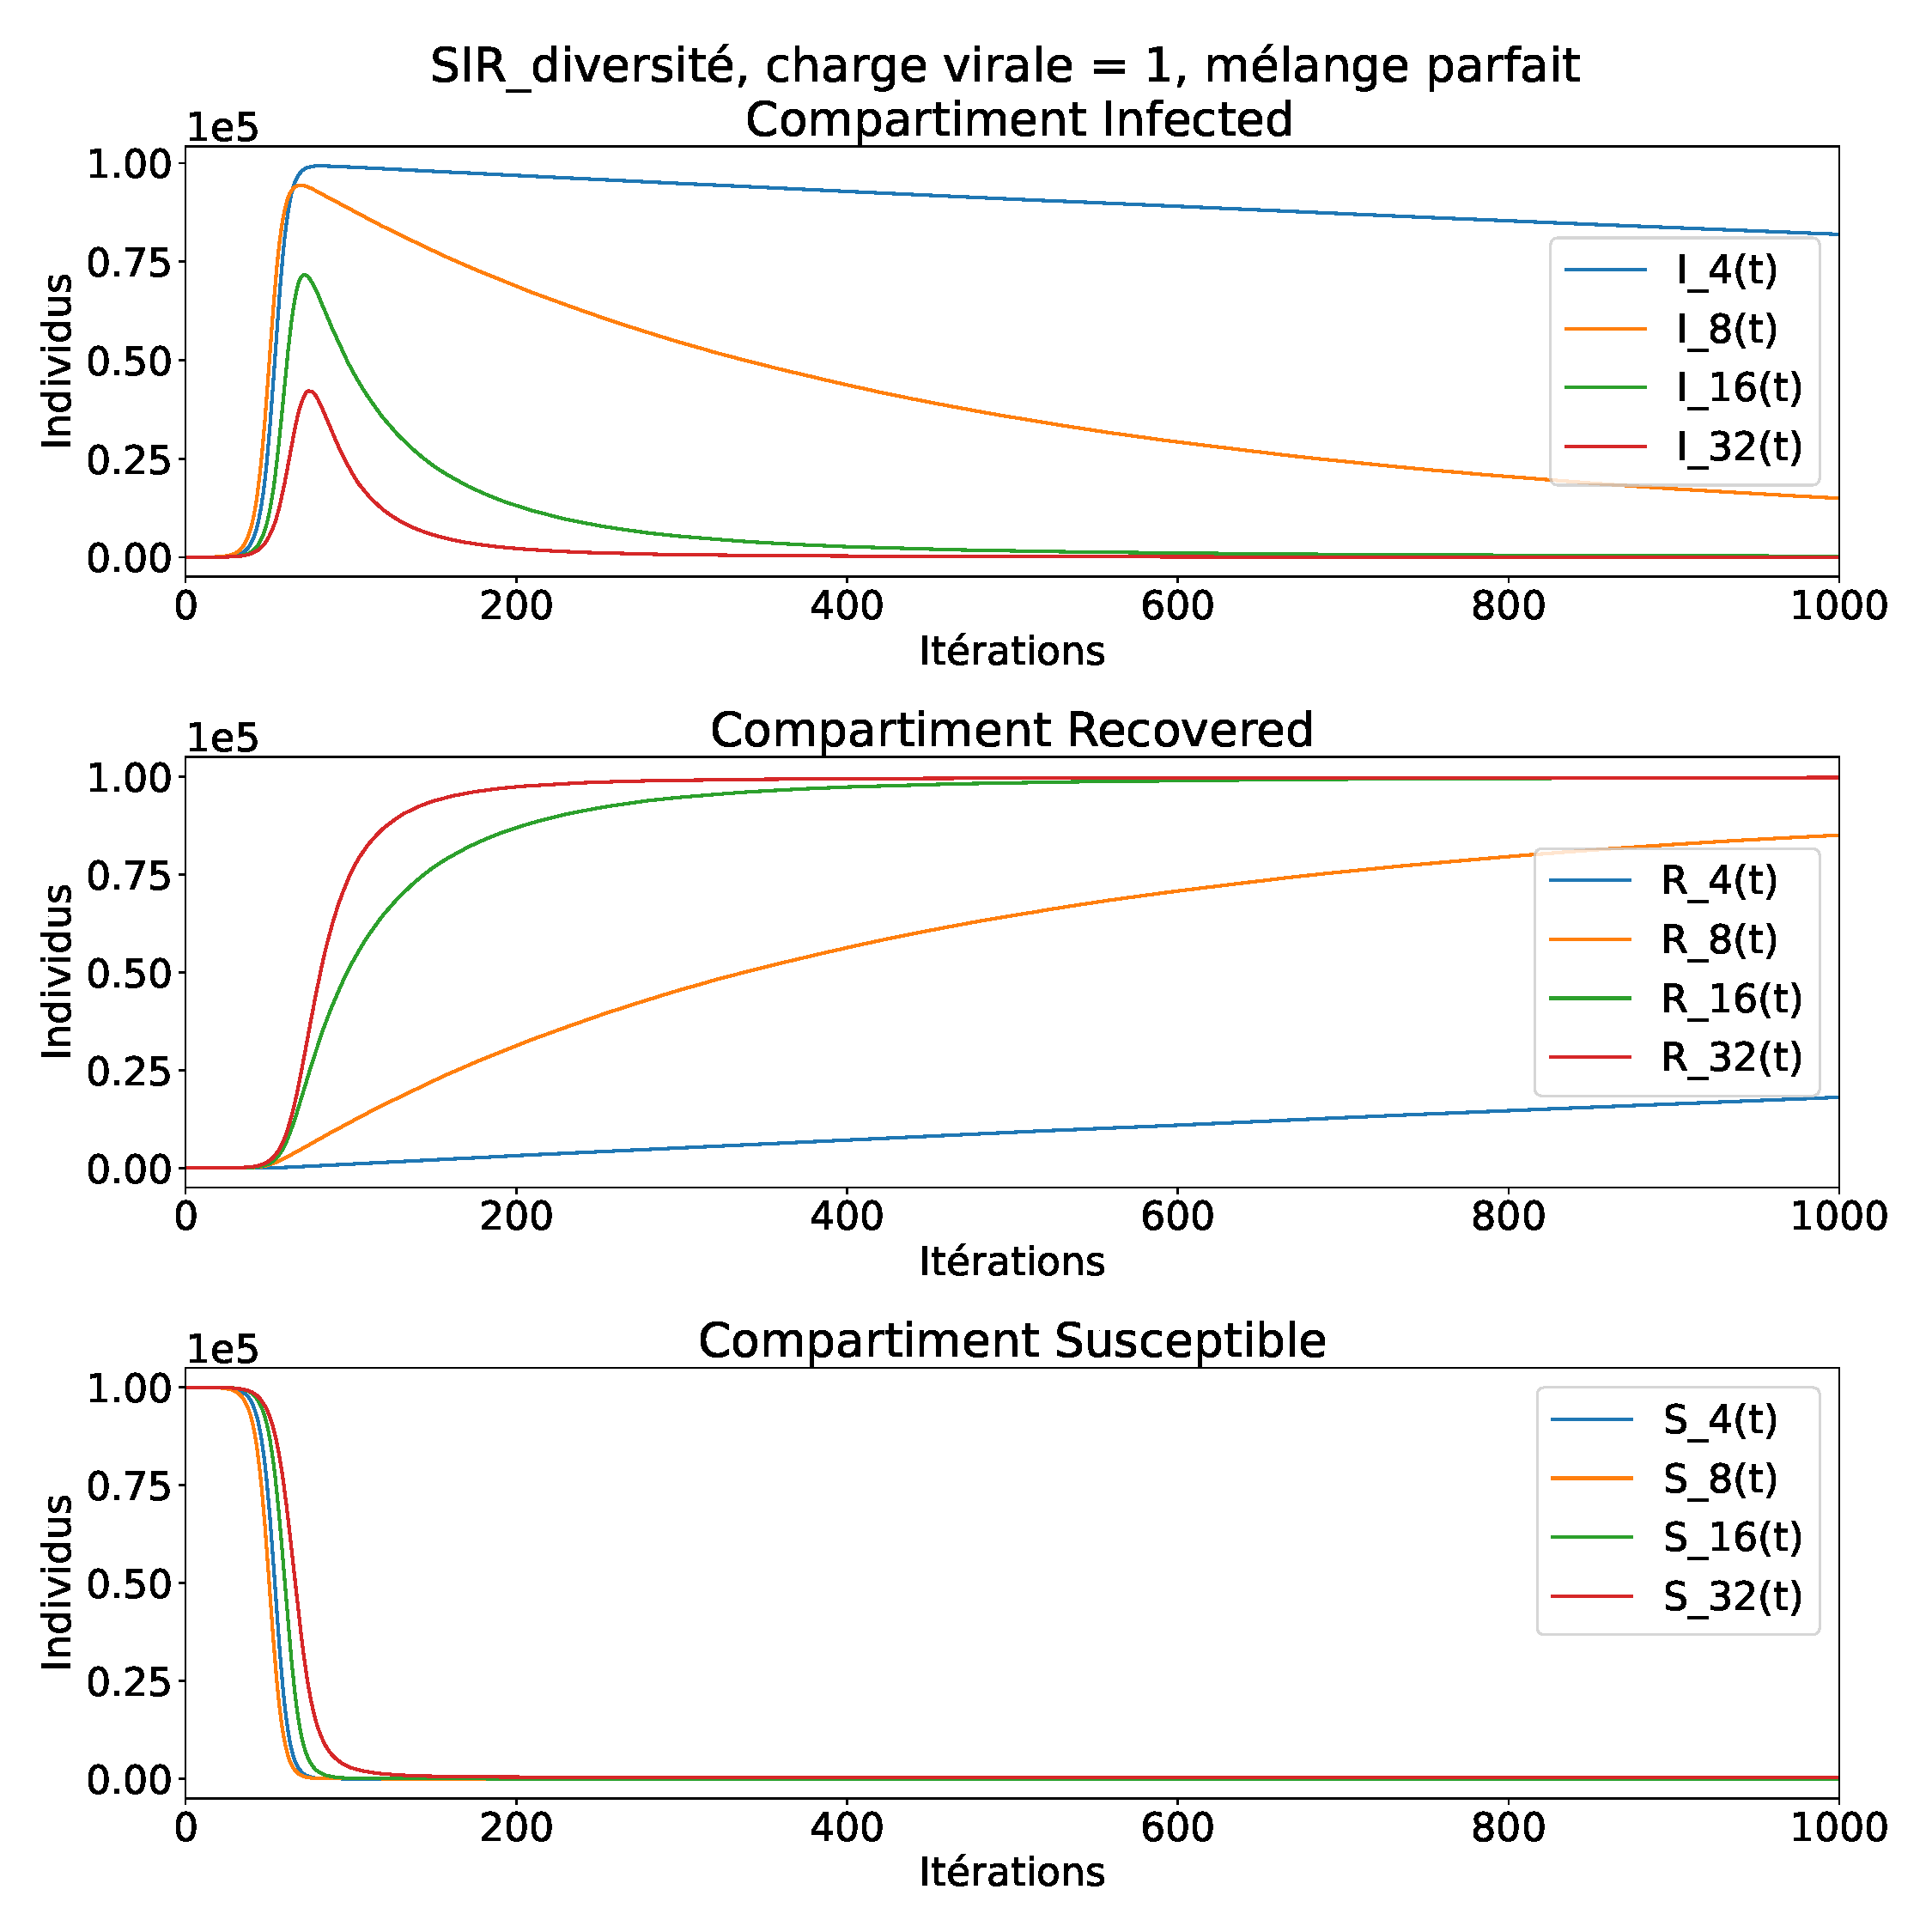
\includegraphics[width=.8\textwidth]{Images/SIR_diversite_mix.pdf}
	\caption[Impacte de la diversité]{Impacte de la diversité d'une population sur une simulation au mélange parfait avec $10^5$ individus et une densité de $1/16$. La première figure montre le compartiment $I$, le second le compartiment $R$ et le dernier le compartiement $S$. Chaque couleur de courbe fait référence à une simulation avec une certaine valeur de diversité notée dans la légende.}
\end{figure}

L'objectif de ce chapitre est d'observer le comportement du système lorsque tous les individus sont contaminés. Un système de denstié $1/16$ avec le mélnage parfait et une charge virale de $1$ propage très rapidement une pandémie. Il s'agit ici de constater les comportements du système lors des immunisation.\\

La première observation est que pour les $4$ simulations, tous les individus quittent rapidement le compartiement $S$ mais ceci légèrement moins rapidement pour les simualtions à forte diversité. Ceci est du au fait qu'une grande diversité produit des individus résistants qui freinent la propagation du pathogène mais l'impacte n'est que léger.\\

La seconde constatation se trouve dans le compartiement $R$. Les individus contaminés s'immunisent plus rapidement dans les systèmes à forte densité. Ce résultat suit l'intuition car les génomes initiaux avantagent l'agent pathogène et donc réduisent la probabilité pour les individus de s'immuniser. Par conséquent, une forte diverstié réduit la compatibilité entre les agent pathogènes et les individus et permettent une immuniations plus rapide.

\section{Taux de pandémies}

Ce chapitre cherche à calculer des statistiques concernant des simulations qui ne développent pas de pandémies. L'objectif est que quantifier l'impacte de la diversité sur le taux de simulations qui donnent ou ne donnent pas de pandémie. Cette section nécessite des statistiques sur un grand nombre de simulations car nous mesurons des événements qui sont très sensibles aux variations.\\

Toutes les configurations étudiées sont de taille $1264	\times 1264$ avec $10^5$ individus. Les simulations ont deux conditions d'arrêt. La première arrive lorsque plus aucun individus n'est contaminé et la seconde survient lorsque $10\%$ de la population a été touchées par la pandémie. Nous estimons qu'à partir de $10\%$, les simulations adopent un comportement purement déterministe.\\

La suite présente des statistiques sur les simulations incluant de la diversité qui n'ont pas développé de pandémie. En effet, nous nous intéressons tout particulièrement aux situations ou une pandémie est évitée. Les données relevées concernant ces simulations sont : le nombre maximum de contaminés simultanément, l'itération de ce maximum, l'itération de fin de simulations (lorsque plus aucun individu n'est contaminé), l'ampleur de la pandémie (nombre de personnes sorties du compartiement $S$) et finalement le taux de simulations qui ont développé une pandémie parmi les $100$ simulations pour chaque configuration.\\

Un total de $64$ configurations de simulations sont étudiées et pour chacune de ces configuration nous effectuons $100$ simulations. L'exécution de $100$ simulations pour un ensemble de paramètres permet de calculer le taux d'événements pandémiques ainsi que de relever les caractéristiques des simulations qui ne font pas apparaitre de pandémie.

\begin{table}[H]
	\centering
	\renewcommand{\arraystretch}{0.6}
	\captionsetup{justification=centering}
	\caption[Taux de succès : diversité 4]{Résultats moyennées des 100 simulations sur un ensemble de $12$ configuration à diversité $4$. Nous mesurons le taux de succès des pandémies ainsi que la taille totale des pandémies qui échouent.\label{tab:grid}}
	\begin{tabular}{@{\extracolsep{\fill} } |c| c| c| c| c|}
		\toprule
		Diversité & charge virale & Mouvements & Succès & Taille pandémie \\
		\midrule
		4         & 1             & 1          & 100\%  & nan             \\
		\midrule
		4         & 1             & 10         & 100\%  & nan             \\
		\midrule
		4         & 1             & 50         & 100\%  & nan             \\
		\midrule
		4         & 0.75          & 1          & 99\%   & 1               \\
		\midrule
		4         & 0.75          & 10         & 100\%  & nan             \\
		\midrule
		4         & 0.75          & 50         & 100\%  & nan             \\
		\midrule
		4         & 0.5           & 1          & 99\%   & 1               \\
		\midrule
		4         & 0.5           & 10         & 100\%  & nan             \\
		\midrule
		4         & 0.5           & 50         & 100\%  & nan             \\
		\midrule
		4         & 0.25          & 1          & 100\%  & nan             \\
		\midrule
		4         & 0.25          & 10         & 98\%   & 1               \\
		\midrule
		4         & 0.25          & 50         & 100\%  & nan             \\
		\bottomrule
	\end{tabular}
\end{table}

Les taux de succès des simulations en diversité $4$ sont dû au fait que l'agent pathogène reste très virulent même avec une distance de hamming maxime de $4$ dans ces configurations. Par conséquent, presques toutes les simulations finissent sur une pandémie.

\begin{table}[H]
	\centering
	\renewcommand{\arraystretch}{0.6}
	\captionsetup{justification=centering}
	\caption[Statistiques : diversité 4]{Résultats moyennées des 100 simulations sur un ensemble de $12$ configuration à diversité $4$. Nous mesurons le maximum d'individus contaminés simultanément, l'itération de ce maximum ainsi que l'itération de la fin de la simulations. A nouveau, nous ne mesurons que pour les simulations qui ne développend pas de pandémie.\label{tab:grid}}
	\begin{tabular}{@{\extracolsep{\fill} } |c| c| c| c| c| c|}
		\toprule
		Diversité & Charge virale & Mouvements & Max & Iteration max & Iteration fin \\
		\midrule
		4         & 1             & 1          & nan & nan           & nan           \\
		\midrule
		4         & 1             & 10         & nan & nan           & nan           \\
		\midrule
		4         & 1             & 50         & nan & nan           & nan           \\
		\midrule
		4         & 0.75          & 1          & 1   & 0             & 24            \\
		\midrule
		4         & 0.75          & 10         & nan & nan           & nan           \\
		\midrule
		4         & 0.75          & 50         & nan & nan           & nan           \\
		\midrule
		4         & 0.5           & 1          & nan & nan           & nan           \\
		\midrule
		4         & 0.5           & 10         & nan & nan           & nan           \\
		\midrule
		4         & 0.5           & 50         & nan & nan           & nan           \\
		\midrule
		4         & 0.25          & 1          & nan & nan           & nan           \\
		\midrule
		4         & 0.25          & 10         & 1   & 0             & 4.5           \\
		\midrule
		4         & 0.25          & 50         & nan & nan           & nan           \\
		\bottomrule
	\end{tabular}
\end{table}

Toutes les configurations qui n'ont pas eu de pandémie déclarée n'ont pas relevé d'informations. Pour les rares simulations à avoir échoué, les échecs se produisent parceque le patient zéro n'est parvenu à contaminer personne.

\begin{table}[H]
	\centering
	\renewcommand{\arraystretch}{0.6}
	\captionsetup{justification=centering}
	\caption[Taux de succès : diversité 8]{Résultats moyennées des 100 simulations sur un ensemble de $12$ configuration à diversité $8$. Nous mesurons le taux de succès des pandémies ainsi que la taille totale des pandémies qui échouent.\label{tab:grid}}
	\begin{tabular}{@{\extracolsep{\fill} } |c| c| c| c| c|}
		\toprule
		Diversité & charge virale & Mouvements & Succès & Taille pandémie \\
		\midrule
		8         & 1             & 1          & 99\%   & 1               \\
		\midrule
		8         & 1             & 10         & 100\%  & nan             \\
		\midrule
		8         & 1             & 50         & 100\%  & nan             \\
		\midrule
		8         & 0.75          & 1          & 98\%   & 1               \\
		\midrule
		8         & 0.75          & 10         & 98\%   & 1.5             \\
		\midrule
		8         & 0.75          & 50         & 99\%   & 1               \\
		\midrule
		8         & 0.5           & 1          & 96\%   & 1               \\
		\midrule
		8         & 0.5           & 10         & 98\%   & 1               \\
		\midrule
		8         & 0.5           & 50         & 98\%   & 1               \\
		\midrule
		8         & 0.25          & 1          & 93\%   & 1               \\
		\midrule
		8         & 0.25          & 10         & 96\%   & 1               \\
		\midrule
		8         & 0.25          & 50         & 94\%   & 1               \\
		\bottomrule
	\end{tabular}
\end{table}

Mêmes observations pour les simulations en diversité $8$. Les taux de succès sont très élevés et les tailles de pandémies sont minimales sur les simulations échouant.

\begin{table}[H]
	\centering
	\renewcommand{\arraystretch}{0.6}
	\captionsetup{justification=centering}
	\caption[Statistiques : diversité 8]{Résultats moyennées des 100 simulations sur un ensemble de $12$ configuration à diversité $8$. Nous mesurons le maximum d'individus contaminés simultanément, l'itération de ce maximum ainsi que l'itération de la fin de la simulations. A nouveau, nous ne mesurons que pour les simulations qui ne développend pas de pandémie.\label{tab:grid}}
	\begin{tabular}{@{\extracolsep{\fill} } |c| c| c| c| c| c|}
		\toprule
		Diversité & Charge virale & Mouvements & Max & Iteration max & Iteration fin \\
		\midrule
		8         & 1             & 1          & 1   &               & 15            \\
		\midrule
		8         & 1             & 10         & nan & nan           & nan           \\
		\midrule
		8         & 1             & 50         & nan & nan           & nan           \\
		\midrule
		8         & 0.75          & 1          & 1   & 0             & 9.5           \\
		\midrule
		8         & 0.75          & 10         & 1.5 & 5.5           & 12            \\
		\midrule
		8         & 0.75          & 50         & 1   & 0             & 9             \\
		\midrule
		8         & 0.5           & 1          & 1   & 0             & 6.75          \\
		\midrule
		8         & 0.5           & 10         & 1   & 0             & 5             \\
		\midrule
		8         & 0.5           & 50         & 1   & 0             & 16            \\
		\midrule
		8         & 0.25          & 1          & 1   & 0             & 31.43         \\
		\midrule
		8         & 0.25          & 10         & 1   & 0             & 9.25          \\
		\midrule
		8         & 0.25          & 50         & 1   & 0             & 11.5          \\
		\bottomrule
	\end{tabular}
\end{table}

Toutes les simulations en diversité $8$ qui ne donnent pas de pandémies sont dû au fait que le patient zéro n'a contaminé personne et le pathogène meurt trop vite.

\begin{table}[H]
	\centering
	\renewcommand{\arraystretch}{0.6}
	\captionsetup{justification=centering}
	\caption[Taux de succès : diversité 16]{Résultats moyennées des 100 simulations sur un ensemble de $12$ configuration à diversité $16$. Nous mesurons le taux de succès des pandémies ainsi que la taille totale des pandémies qui échouent.\label{tab:grid}}
	\begin{tabular}{@{\extracolsep{\fill} } |c| c| c| c| c|}
		\toprule
		Diversité & charge virale & Mouvements & Succès & Taille pandémie \\
		\midrule
		16        & 1             & 1          & 81\%   & 1.32            \\
		\midrule
		16        & 1             & 10         & 90\%   & 1               \\
		\midrule
		16        & 1             & 50         & 100\%  & nan             \\
		\midrule
		16        & 0.75          & 1          & 75\%   & 3.04            \\
		\midrule
		16        & 0.75          & 10         & 87\%   & 1.15            \\
		\midrule
		16        & 0.75          & 50         & 90\%   & 1.1             \\
		\midrule
		16        & 0.5           & 1          & 59\%   & 4.88            \\
		\midrule
		16        & 0.5           & 10         & 86\%   & 1.36            \\
		\midrule
		16        & 0.5           & 50         & 88\%   & 1.17            \\
		\midrule
		16        & 0.25          & 1          & 1\%    & 816.92          \\
		\midrule
		16        & 0.25          & 10         & 67\%   & 1.76            \\
		\midrule
		16        & 0.25          & 50         & 72\%   & 1.32            \\
		\bottomrule
	\end{tabular}
\end{table}

L'impace de la diversité apparait à partir d'une diversité de $16$. Naturellement, le nombre de mouvement impacte grandement la réussite d'une pandémie et ceci est perçu dans les taux de réussite. Les taux de réussite de la table au dessus sont nettement plus faibles que pour les mêmes simulations aux diversités inférieures mais la taille des pandémies reste très faible sauf pour une configuration. Généralement les simulations à cette diversité échouent sans se propager du tout mais la simulation de diverstié $16$, charge virale $0.25$ et le nombre de mouvement de $1$ montre des comportement étonnants.\\

Presque toutes les simulations de cette configuration ont échoué et ceci avec une taille de pandémie moyenne de plus de $816$ individus. C'est pour l'instant la seule configuration à montrer des plus grandes pandémies mais qui finissent quand même par échouer.

\begin{table}[H]
	\centering
	\renewcommand{\arraystretch}{0.6}
	\captionsetup{justification=centering}
	\caption[Statistiques : diversité 16]{Résultats moyennées des 100 simulations sur un ensemble de $12$ configuration à diversité $16$. Nous mesurons le maximum d'individus contaminés simultanément, l'itération de ce maximum ainsi que l'itération de la fin de la simulations. A nouveau, nous ne mesurons que pour les simulations qui ne développend pas de pandémie.\label{tab:grid}}
	\begin{tabular}{@{\extracolsep{\fill} } |c| c| c| c| c| c|}
		\toprule
		Diversité & Charge virale & Mouvements & Max   & Iteration max & Iteration fin \\
		\midrule
		16        & 1             & 1          & 1.21  & 1.37          & 12.37         \\
		\midrule
		16        & 1             & 10         & 1     & 0             & 5.3           \\
		\midrule
		16        & 1             & 50         & nan   & nan           & nan           \\
		\midrule
		16        & 0.75          & 1          & 2.32  & 8.32          & 31.52         \\
		\midrule
		16        & 0.75          & 10         & 1.15  & 0.46          & 7.23          \\
		\midrule
		16        & 0.75          & 50         & 1.1   & 0.2           & 5.4           \\
		\midrule
		16        & 0.5           & 1          & 2.17  & 16.90         & 51.34         \\
		\midrule
		16        & 0.5           & 10         & 1.36  & 0.71          & 7.21          \\
		\midrule
		16        & 0.5           & 50         & 1.17  & 0.17          & 14.5          \\
		\midrule
		16        & 0.25          & 1          & 28.05 & 989.47        & 2632.66       \\
		\midrule
		16        & 0.25          & 10         & 1.58  & 6.91          & 25.88         \\
		\midrule
		16        & 0.25          & 50         & 1.21  & 3.07          & 15.82         \\
		\bottomrule
	\end{tabular}
\end{table}

De toutes les simulations qui ont échouée, seule une persiste et parvient à contaminer un maximum de $28$ individus en moyenne et finit par s'achever à $2632$ itérations en moyenne.

\begin{table}[H]
	\centering
	\renewcommand{\arraystretch}{0.6}
	\captionsetup{justification=centering}
	\caption[Taux de succès : diversité 32]{Résultats moyennées des 100 simulations sur un ensemble de $12$ configuration à diversité $32$. Nous mesurons le taux de succès des pandémies ainsi que la taille totale des pandémies qui échouent.\label{tab:grid}}
	\begin{tabular}{@{\extracolsep{\fill} } |c| c| c| c| c|}
		\toprule
		Diversité & charge virale & Mouvements & Succès & Taille pandémie \\
		\midrule
		32        & 1             & 1          & 0\%    & 18.02           \\
		\midrule
		32        & 1             & 10         & 72\%   & 1.36            \\
		\midrule
		32        & 1             & 50         & 100\%  & nan             \\
		\midrule
		32        & 0.75          & 1          & 0\%    & 13.46           \\
		\midrule
		32        & 0.75          & 10         & 67\%   & 1.97            \\
		\midrule
		32        & 0.75          & 50         & 76\%   & 1.63            \\
		\midrule
		32        & 0.5           & 1          & 0\%    & 10.98           \\
		\midrule
		32        & 0.5           & 10         & 49\%   & 2.31            \\
		\midrule
		32        & 0.5           & 50         & 43\%   & 1.58            \\
		\midrule
		32        & 0.25          & 1          & 0\%    & 4.56            \\
		\midrule
		32        & 0.25          & 10         & 0\%    & 180.12          \\
		\midrule
		32        & 0.25          & 50         & 19\%   & 3.23            \\
		\bottomrule
	\end{tabular}
\end{table}

Finalement les configurations en diverstié $32$ montrent les taux les plus faibles. Toutes les configurations à $1$ mouvement n'ont donné aucune pandémie et ceci contrairement aux mêmes configurations à diverstié inférieure.

\begin{table}[H]
	\centering
	\renewcommand{\arraystretch}{0.6}
	\captionsetup{justification=centering}
	\caption[Statistiques : diversité 32]{Résultats moyennées des 100 simulations sur un ensemble de $12$ configuration à diversité $32$. Nous mesurons le maximum d'individus contaminés simultanément, l'itération de ce maximum ainsi que l'itération de la fin de la simulations. A nouveau, nous ne mesurons que pour les simulations qui ne développend pas de pandémie.\label{tab:grid}}
	\begin{tabular}{@{\extracolsep{\fill} } |c| c| c| c| c| c|}
		\toprule
		Diversité & Charge virale & Mouvements & Max  & Iteration max & Iteration fin \\
		\midrule
		32        & 1             & 1          & 5.1  & 40.09         & 104.05        \\
		\midrule
		32        & 1             & 10         & 1.25 & 0.68          & 6.32          \\
		\midrule
		32        & 1             & 50         & nan  & nan           & nan           \\
		\midrule
		32        & 0.75          & 1          & 3.99 & 37.93         & 103.11        \\
		\midrule
		32        & 0.75          & 10         & 1.39 & 1.03          & 9.03          \\
		\midrule
		32        & 0.75          & 50         & 1.46 & 1.54          & 7.46          \\
		\midrule
		32        & 0.5           & 1          & 3    & 34.47         & 100.25        \\
		\midrule
		32        & 0.5           & 10         & 1.65 & 4.63          & 14.31         \\
		\midrule
		32        & 0.5           & 50         & 1.29 & 2.86          & 10.91         \\
		\midrule
		32        & 0.25          & 1          & 2.11 & 19.64         & 51.55         \\
		\midrule
		32        & 0.25          & 10         & 7.12 & 145.94        & 245.44        \\
		\midrule
		32        & 0.25          & 50         & 1.88 & 10.67         & 26.51         \\
		\bottomrule
	\end{tabular}
\end{table}

A nouveau, une grande majorité des configuration à diverstié $32$ ne montre des pandémies qui ne naissent pas avec des maximums de contaminés de l'ordre d'une dixaine et une fin de simulations très rapide.

\subsection{Conclusion des résultats}

Les résultats permettent d'observer l'impacte de la diversité sur les systèmes. Apparemment il n'y a pas d'impacte sur la propagation de la pandémie mais uniquement sur la vitesse d'immunisation des individus. Nous cherchions à observer des pandémies qui évoluaient jusqu'à un certain point et dissparaissait ensuite mais ce comportement n'est pas présent dans les mesures.\\

L'absence de ces événements est dû au fonctionnement du modèle et à la notion de diversité. Le problème est que dans le modèle, la diversité n'a aucun impacte sur le propagation de pandémie. Pour rappel, lorsqu'un individu sain est en contact avec un agent pathogène, l'individu devient contaminé et contagieux directement et ceci peu importe la diversité du système. Le seul effet de la diverstié est le fait que cet individu peut s'immuniser plus ou moins rapidement en fonction de cette diversité. Mais le problème est que la propagation se présente sous forme de vague, comme une onde. L'illustration ci-dessous illustre le phénomène.

\newpage

\begin{figure}[h]
	\centering
	\captionsetup{justification=centering}
	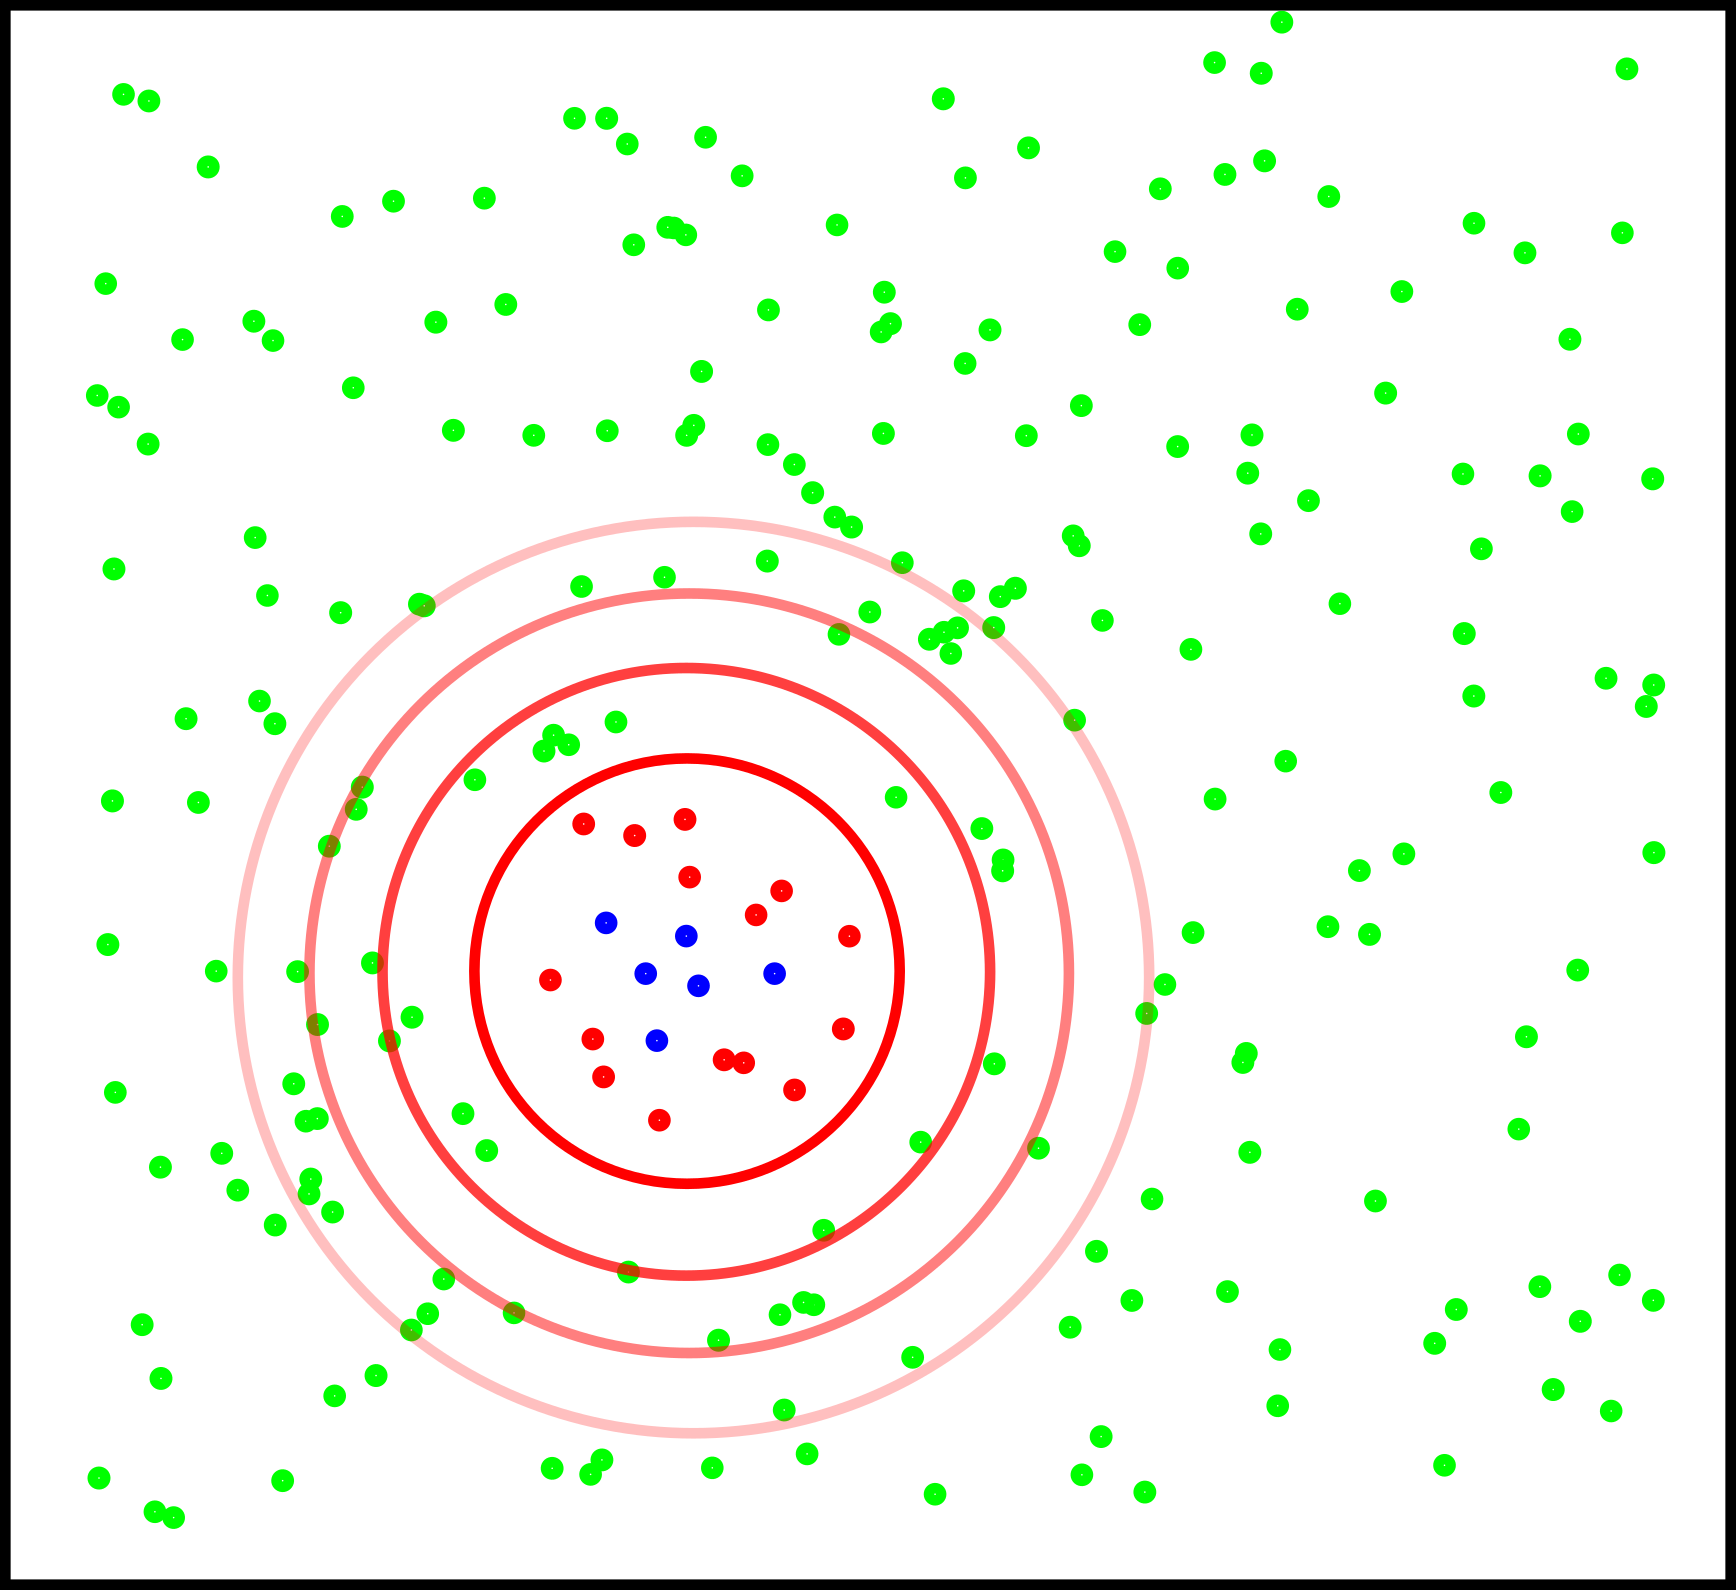
\includegraphics[width=.5\textwidth]{Images/vague_propagation.png}
	\caption{vague propagation}
\end{figure}

La figure montre la propagation d'une pandémie. En vert nous avons les individus sains, en bleu les individus immunisés et en rouge les individus contaminés. Les cercles représentent la propagation de la pandémie sous forme de vagues. Nous pourrion découper le processus en 3 zones distinctes et indépendantes. Le première est la zone centrale du cercle avec les individus immunisés. La seconde est la frontière entre les individus infectés et les sains donc la vague (cercle rouge) et finalement la troisième zone est le reste du système avec uniquement des individus sains.\\

D'après les résultats des simulations, la diversité n'impacte pas la propagation de la pandémie. En effet, la diversité permet l'immunisation plus rapide de la population donc l'apparition davantages de cercles bleus sur l'image. Le problème est que cette première zone est indépendante de la deuxième qui est la vague car cette dernière est beaucoup plus rapide que l'immunisation. Un individu fraichement contaminé propagera la pandémie bien avant qu'il ne s'immunise. Par conséquent, l'ampleur des immunisation n'impacte pas la propagation de la pandémie.\\

Donc la première zone n'affecte pas la vague mais qu'en est-il de la troisième zone ? En réalité la troisième zone est purement uniforme. Si une vague parvient à un moment donné à se propager dans la troisième zone alors elle le pourra jusqu'à contaminer tous les individus.\\

La rélexion mène donc à expliquer que une pandémie se propage soit complètement soit pas du tout.\\

En épidémiologie, le nombre de reproduction de base $R_0$ représente le nombre moyen de contaminations par un individu contaminé. Si ce taux est au dessous de $1$, cela signifie que la pandémie est mourante par contre si le taux est au dessus de $1$, la pandémie se propage.\\

Dans le modèle implémenté et d'après les mesures de diversité, une simulations ne peut pas avoir un $R_0$ qui varie. Cette valeur est fixe du début à la fin. Par conséquent, toutes les simulations au $R_0 < 1$ ne montrent aucune pandémie et au contraire toutes les simulations au $R_0 > 1$ finissent par contaminer tout le monde. Dans une situation réelle, des mesures sanitaires permettent de faire varier ce taux au cours de la propagation de la pendémie. Dans le modèle ce fonctionnement est non présent. Une autre chose n'est pas présente et donc impossible dans le modèle est l'effet d'immunité collective.\\

L'immunité collective est le fait le niveau d'immunité général est siffisemment élevé afin de faire passer le taux $R_0$ en dessous de $1$ et que la pandémie disparaisse. Ce phénomène peut s'obtenir par trois façons. La première est la vaccination, la seconde est l'immunité croisée et la troisième est une forme de résistance naturelle. Si nous reprenions la figure ci-dessus, l'immunité collective dans le modèle pourraient être obtenue d'une seule façon. Il faudrait pouroivr modifier l'état de la troisième zone (les parties du système non contaminés). Si au fil du temps nous pouvions vacciner des individus ou les immuniser en amont de la pandémie alors nous pourrions influencer le $R_0$ de la simulation mais le modèle n'inclut pas ces mécanismes. Par conséquent le $R_0$ reste constant dû à l'homogénéité de la troisième zone.

\section{Pandémies partielles}

\begin{table}[H]
	\centering
	\renewcommand{\arraystretch}{0.6}
	\captionsetup{justification=centering}
	\caption[1]{1\label{tab:grid}}
	\begin{tabular}{@{\extracolsep{\fill} } |c| c| c|}
		\toprule
		Charge virale & Diversité & Taille pandémie \\
		\midrule
		1             & 4         & 100000               \\
		\midrule
		1             & 8         & 100000              \\
		\midrule
		1             & 16        & 99922.68              \\
		\midrule
		1             & 20        & 98699.38              \\
		\midrule
		1             & 24        & 95390.15              \\
		\midrule
		1             & 28        & 91217.14              \\
		\midrule
		1             & 32        & 87863.19              \\
		\midrule
		1             & 36        & 85895.91              \\
		\midrule
		1             & 40        & 85180.41              \\
		\midrule
		1             & 1000      & 86335.36              \\
		\bottomrule
	\end{tabular}
\end{table}

\begin{table}[H]
	\centering
	\renewcommand{\arraystretch}{0.6}
	\captionsetup{justification=centering}
	\caption[1]{1\label{tab:grid}}
	\begin{tabular}{@{\extracolsep{\fill} } |c| c| c|}
		\toprule
		Charge virale & Diversité & Taille pandémie \\
		\midrule
		0.75             & 4         & 100000               \\
		\midrule
		0.75             & 8         & 100000              \\
		\midrule
		0.75             & 16        & 99519.62              \\
		\midrule
		0.75             & 20        & 95731.53              \\
		\midrule
		0.75             & 24        & 88009.51              \\
		\midrule
		0.75             & 28        & 79550.08              \\
		\midrule
		0.75             & 32        & 73206.16              \\
		\midrule
		0.75             & 36        & 69406.5              \\
		\midrule
		0.75             & 40        & 68092.52              \\
		\midrule
		0.75             & 1000      & 70344.02              \\
		\bottomrule
	\end{tabular}
\end{table}

\begin{table}[H]
	\centering
	\renewcommand{\arraystretch}{0.6}
	\captionsetup{justification=centering}
	\caption[1]{1\label{tab:grid}}
	\begin{tabular}{@{\extracolsep{\fill} } |c| c| c|}
		\toprule
		Charge virale & Diversité & Taille pandémie \\
		\midrule
		0.5             & 4         & 100000               \\
		\midrule
		0.5             & 8         & 100000              \\
		\midrule
		0.5             & 16        & 96823.41              \\
		\midrule
		0.5             & 20        & 84180.41              \\
		\midrule
		0.5             & 24        & 64485.21              \\
		\midrule
		0.5             & 28        & 43646.63              \\
		\midrule
		0.5             & 32        & 23020.03              \\
		\midrule
		0.5             & 36        & 11854.48              \\
		\midrule
		0.5             & 40        & 7983.12              \\
		\midrule
		0.5             & 1000      & 11401.21              \\
		\bottomrule
	\end{tabular}
\end{table}
